\chapter{Introducción Específica} % Main chapter title

\label{Chapter2}

%----------------------------------------------------------------------------------------
%	SECTION 1
%----------------------------------------------------------------------------------------
En este capitulo se muestra la idea general del proyecto y se describen las características principales de la solución implementada.
\section{Estructura general del sistema}

%\label{sec:ejemplo}

El diagrama general del sistema se muestra en figura \ref{fig:esquemaGeneral}. El sistema se compone de un microcontrolador ARM(\textit{Advanced RISC Machine}) Cortex\textregistered -M4 y dos bus UART(\textit{Universal Asynchronous Receiver-Transmitter}) para que el sistema pueda tener una arquitectura modular que le permite incorporar nuevas tecnologías de comunicación para transmitir inalambricamente tales como: SigFox, LoRa, Nb-IOT, Cat-M, WiFi y 3G.


\begin{figure}[h]

	\centering

	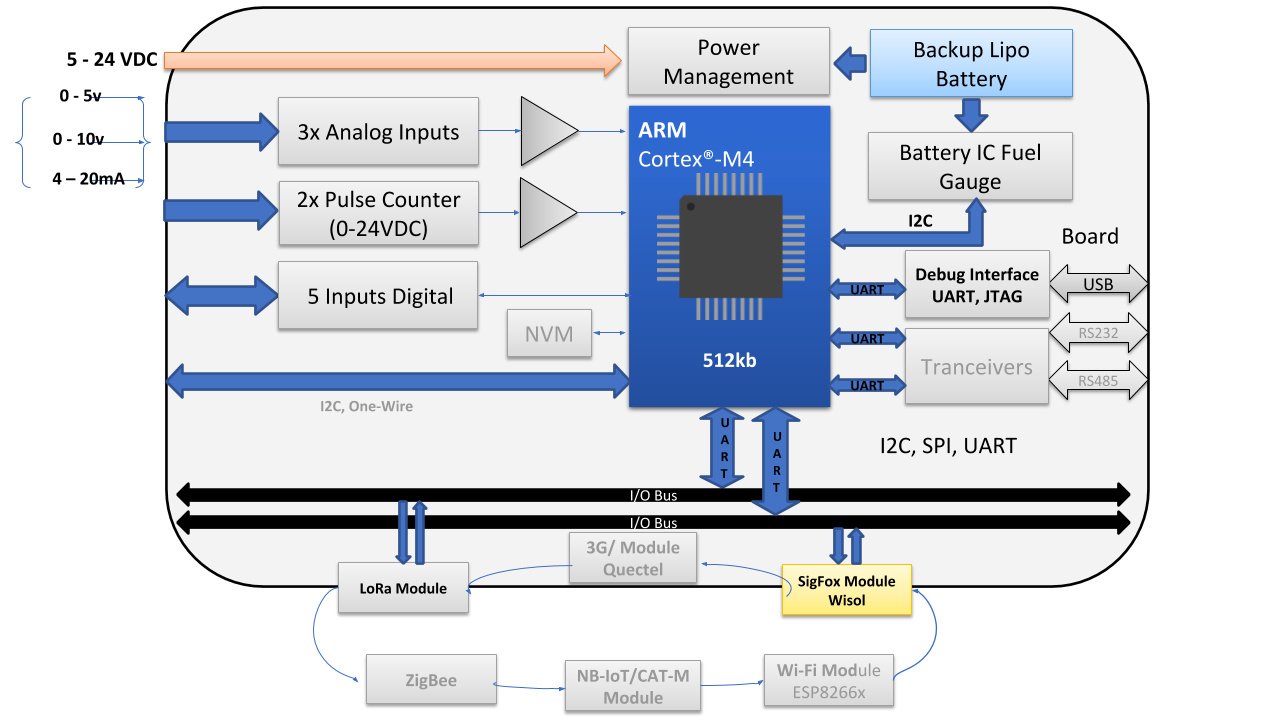
\includegraphics[scale=.35]{./Figures/esquemaGeneral.png}

	\caption{Diagrama general del sistema.}

	\label{fig:esquemaGeneral}

\end{figure}


El sistema consta de un medidor de voltaje para batería de LiPo, dos entradas analógicas de tensión, una de corriente y cinco entradas digitales con el fin de poder adquirir datos de diferentes variables en los procesos industriales. El dispositivo esta diseñado para tener diferentes funcionalidades sin embargo debido a la delimitación del alcance del trabajo no se tubo en cuenta los subsitemas que se observan en gris en la figura \ref{fig:esquemaGeneral}.


\section{Requerimientos}
Los siguientes son los requerimientos del presente trabajo:

\textbf{Grupo de requerimientos asociados al hardware:}
\begin{enumerate}

	\item Microcontrolador.

	\begin{itemize}

		\item Debe tener procesador ARM Cortex M0+ o M4.

		\item Debe tener 3 puertos UART.

		\item Debe tener comunicación I2C/SPI.

		\item Debe tener memoria flash mayor a 64 kb.

		\item Debe tener 3 entradas analógicas.

		\item Debe tener 5 entradas digitales.

	\end{itemize}

	%\item Nivel de protección debe ser IP65.

	\item Autonomía de la batería debe ser de 1 días.

	\item Módulo Sigfox.

		\begin{itemize}

			\item Debe tener un módulo Dual Zone con comunicación por UART.

			\item Debe tener antena externa con centro de banda en 915 MHz.

		\end{itemize}

	\item Módulo Lora.

		\begin{itemize}

			\item Debe tener un módulo con comunicación por UART/I2C.

			\item Debe tener antena externa con centro de banda en 915 MHz.

		\end{itemize}

		\item El sistema debe tener una (1) entrada analógica de voltaje de 0-5 Vdc.
		
		\item El sistema debe tener una (1) entrada analógica de voltaje de 0-10 Vdc.

		\item El sistema debe tener una (1) entradas analógicas de corriente 4-20 mA.

		\item El sistema debe tener cinco (5) entradas digitales 3.3-24 Vdc.

\end{enumerate}



\textbf{Grupo de requerimientos asociados al módulo Sigfox:}

	\begin{enumerate}

		\item Debe colocarse en modo de bajo consumo mientras no esté en uso.

		\item Transmisiones Uplink al backend de sigfox máximo 50 mensajes por día.

		\item Verificación de cada respuesta de comando AT enviado desde el MCU al módulo SIgFox.

	\end{enumerate}





\textbf{Grupo de requerimientos asociados al módulo Lora:}

	\begin{enumerate}

		\item Verificación de cada respuesta de los comandos enviados desde el MCU al módulo Lora.

		\item Debe colocarse en modo de bajo consumo mientras no esté en uso.

	\end{enumerate}



\textbf{Otros requerimientos:}

\begin{enumerate}

	\item En el sistema se podrán configurar umbrales máximos y mínimos de las lecturas analógicas.

	\item El sistema deberá verificar las entradas analógicas cada 1 minuto (parámetro configurable).

	\item El sistema saldrá del modo de bajo consumo cada vez que ocurra una interrupción externa.

\end{enumerate}



\subsection{Sigfox}
Contexto y explicación  completo de que es Sigfox...
Contexto y explicación  completo de que es Sigfox...
Contexto y explicación  completo de que es Sigfox...
\subsection{Lora}
Contexto y explicacióncompleto de que es Lora...

%\section{Antecedentes}

Si se desea indicar alguna página web utilizar el siguiente formato de referencias bibliográficas, dónde las referencias se detallan en la sección de bibliografía de la memoria,utilizado el formato establecido por IEEE en \citep{IEEE:citation}. Por ejemplo, ``el presente trabajo se basa en la plataforma EDU-CIAA-NXP, la cual se describe en detalle en \citep{CIAA}''.

\subsection{Figuras} 

La forma correcta de utilizar una figura es la siguiente: ``Se eligió utilizar un cuadrado azul para el logo, el cual se ilustra en la figura \ref{fig:esquemaGeneral}''.

%\begin{figure}[h]
%	\centering
%	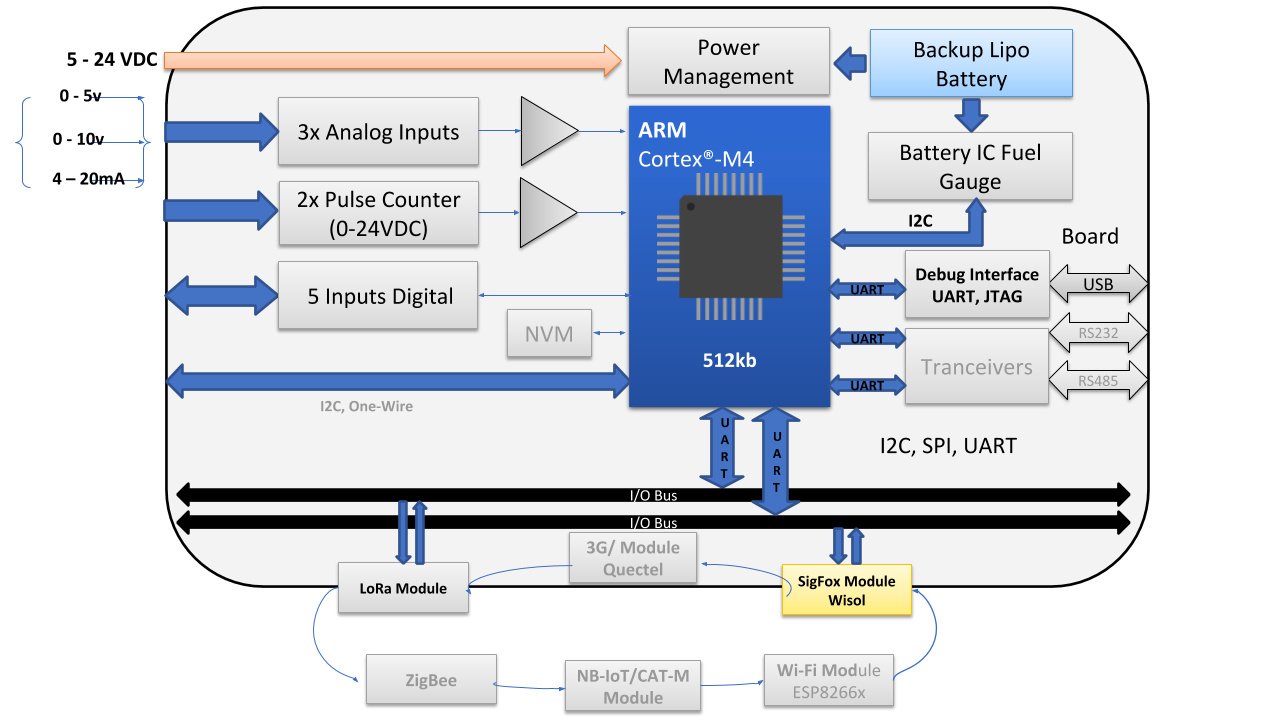
\includegraphics[scale=.35]{./Figures/esquemaGeneral.png}
%	\caption{Diagrama general del sistema.}
%	\label{fig:esquemaGeneral}
%\end{figure}

El texto de las figuras debe estar siempre en español, excepto que se decida reproducir una figura original tomada de alguna referencia. En ese caso la referencia de la cual se tomó la figura debe ser indicada en el epígrafe de la figura e incluida como una nota al pie, como se ilustra en la figura \ref{fig:palabraIngles}.

\begin{figure}[h!]
	\centering
	
\includegraphics[scale=.25]{./Figures/word.jpeg}
	\caption{Imagen tomada de la página oficial del procesador\protect\footnotemark.}
	\label{fig:palabraIngles}
\end{figure}

\footnotetext{\url{https://goo.gl/images/i7C70w}}


La figura y el epígrafe deben conformar una unidad cuyo significado principal pueda ser comprendido por el lector sin necesidad de leer el cuerpo central de la memoria. Para eso es necesario que el epígrafe sea todo lo detallado que corresponda y si en la figura se utilizan abreviaturas entonces aclarar su significado en el epígrafe o en la misma figura.

\begin{figure}[h]
	\centering
	
\includegraphics[scale=.4]{./Figures/questionMark.png}
	\caption{El lector no sabe por qué de pronto aparece esta figura.}
	\label{fig:questionMark}
\end{figure}

Nunca colocar una figura en el documento antes de hacer la primera referencia a ella, como se ilustra con la figura \ref{fig:questionMark}, porque sino el lector no comprenderá por qué de pronto aparece la figura en el documento, lo que distraerá su atención.

\subsection{Ecuaciones}
\label{sec:Ecuaciones}

Al insertar ecuaciones en la memoria estas se deben numerar de la siguiente forma:

\begin{equation}
	\label{eq:metric}
	ds^2 = c^2 dt^2 \left( \frac{d\sigma^2}{1-k\sigma^2} + \sigma^2\left[ d\theta^2 + \sin^2\theta d\phi^2 \right] \right)
\end{equation}
                                                        
Es importante tener presente que en el caso de las ecuaciones estas pueden ser referidas por su número, como por ejemplo ``tal como describe la ecuación \ref{eq:metric}'', pero también es correcto utilizar los dos puntos, como por ejemplo ``la expresión matemática que describe este comportamiento es la siguiente:''

\begin{equation}
	\label{eq:schrodinger}
	\frac{\hbar^2}{2m}\nabla^2\Psi + V(\mathbf{r})\Psi = -i\hbar \frac{\partial\Psi}{\partial t}
\end{equation}

Para las ecuaciones se debe utilizar un tamaño de letra equivalente al utilizado para el texto del trabajo, en tipografía cursiva y preferentemente del tipo Times New Roman o similar. El espaciado antes y después de cada ecuación es de aproximadamente el doble que entre párrafos consecutivos del cuerpo principal del texto. Por suerte la plantilla se encarga de esto por nosotros.

Para generar la ecuación \ref{eq:metric} se utilizó el siguiente código:

\begin{verbatim}
\begin{equation}
	\label{eq:metric}
	ds^2 = c^2 dt^2 \left( \frac{d\sigma^2}{1-k\sigma^2} + 
	\sigma^2\left[ d\theta^2 + 
	\sin^2\theta d\phi^2 \right] \right)
\end{equation}
\end{verbatim}

Y para la ecuación \ref{eq:schrodinger}:

\begin{verbatim}
\begin{equation}
	\label{eq:schrodinger}
	\frac{\hbar^2}{2m}\nabla^2\Psi + V(\mathbf{r})\Psi = 
	-i\hbar \frac{\partial\Psi}{\partial t}
\end{equation}

\end{verbatim}